\chapter{Securing LAN}

\section{Port security}

\textbf{CAM table overflow} attacks (also called MAC address overflow attacks) take place by bombarding the switch with fake source MAC addresses until the switch MAC address table is full. If enough entries are entered into the CAM table, the table fills up to the point that no new entries can be accepted. When this occurs, the switch treats the frame as an unknown unicast and begins to flood all incoming traffic to all ports. As a result, the attacker can capture all of the frames sent from one host to another.\\

The simplest and most effective method to prevent CAM table overflow attacks is to enable \textbf{port security}. When a port configured with port security receives a frame, the source MAC address of the frame is compared to the list of secure source addresses that were manually configured or autoconfigured (learned) on the port.\\

To enable port security, use the \code{sw port-security} interface configuration command on an access port. Notice that, the port must be configured as an access port before port security can be enabled. This is because port security can only be configured on access ports and, by default, Layer 2 switch ports are set to dynamic auto (trunking on). Therefore, the port must be initially configured with the \code{sw mode access} interface configuration command.\\

To set the maximum number of MAC addresses allowed on a port use the \code{sw port-security max <value>}.\\

A security \textbf{violation} is created when a station with a MAC address that is not in the address table attempts to access the interface when the table is full. Another example of a situation that creates a security violation is when an address is being used on two secure interfaces in the same VLAN. If a MAC address of a device attached to the port differs from the list of secure addresses, then a port violation occurs, and the port enters the error-disabled state.\\

To set the port security violation mode, use the \code{sw port-security violation {protect | restrict | shutdown | shutdown vlan}} interface configuration command. To re-enable an error-disable port, manually re-enable the disabled port by entering the \code{shutdown} and \code{no shutdown} interface configuration commands. Alternatively, the switch could be configured to automatically re-enable an error-disabled port using the \code{errdisable recovery cause psecure-violation} global configuration mode command.\\

Port security aging  remove secure MAC addresses on a secure port without manually deleting the existing secure MAC addresses. Use the \code{sw port-security aging} command to enable or disable static aging for the secure port, or to set the aging time or type. Two types of aging are supported per port:

\begin{itemize}
\item Absolute -- The secure addresses on the port are deleted after the specified aging time.
\item Inactivity -- The secure addresses on the port are deleted only if they are inactive for the specified aging time.
\end{itemize}

The \textbf{MAC address notification} feature sends SNMP traps to the network management station (NMS) whenever a new MAC address is added to, or an old address is deleted from the forwarding tables. MAC address notifications are generated only for dynamic and secure MAC addresses. Use the \code{mac address-table notification} global configuration command to enable the MAC address notification feature on a switch.

\section{DTP, trunking and access mode}

A \textbf{VLAN hopping attack} enables traffic from one VLAN to be seen by another VLAN without the aid of a router. A VLAN hopping attack can be launched in one of two ways:

\begin{itemize}
\item Spoofing DTP messages from the attacking host to cause the switch to enter trunking mode. From here, the attacker can send traffic tagged with the target VLAN, and the switch then delivers the packets to the destination.
\item Introducing a rogue switch and enabling trunking. The attacker can then access all the VLANs on the victim switch from the rogue switch.
\end{itemize}

\textbf{Double-tagging} takes advantage of 802.1Q de-encapsulation, in which the attacker adds a hidden 802.1Q tag inside the frame. This tag allows the frame to go to another VLAN. For example, an attacker on VLAN 10 tags a frame for VLAN 10 and inserts an additional tag for VLAN 20.  An important characteristic of the double-encapsulated VLAN hopping attack is that it works even if trunk ports are disabled, as a host typically sends a frame on a segment that is not a trunk link. \\

The best way to prevent basic VLAN hopping attacks:

\begin{itemize}
\item Manually enable trunking and access ports
\item Disable DTP
\item Be sure that native VLAN is only used for trunk lines.
\end{itemize}

\section{Priavte VLAN}

Private VLANs (PVLAN) provide Layer 2 isolation between hosts within the same VLAN. There are three types of PVLAN ports (figure \ref{PVLAN}):

\begin{itemize}
\item A \textbf{promiscuous} port can talk to everyone. This is often the port connected to the router.
\item An \textbf{isolated} port can only talk to promiscuous ports. If you want to isolate hosts within the same VLAN, configure them as isolated port.
\item \textbf{Community} ports can talk to ports in the same community and promiscuous ports.
\end{itemize}

\begin{figure}[hbtp]
\caption{PVLANs -- promiscuous ports, isolated ports, community ports}\label{PVLAN}
\centering
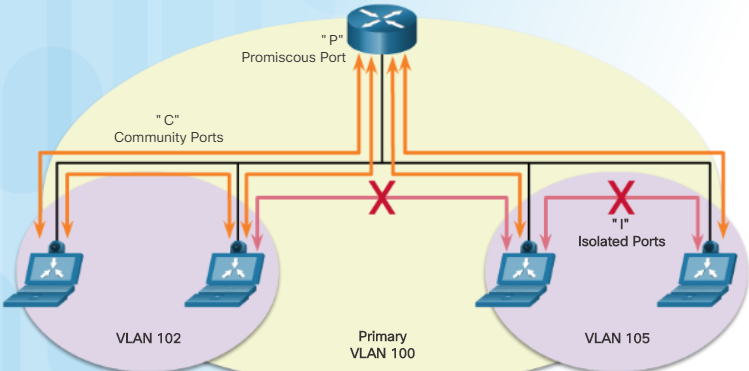
\includegraphics[scale=0.5]{pictures/PVLAN.PNG}
\end{figure}

Full PVLAN support is available on 3560 Multiplayer switches or higher. The 2960 Switches only support a part of PVLAN (PVLAN Edge). \\

In creating full PVLAN, you need to create three special VLANs: primary VLAN (goes with the promiscuous ports), isolated VLAN, and community VLAN (can be different communities based on the VLAN number). Look at the figure \ref{PVLANconfig} for sample configuration. In order for PVLAN to work, you need to set VTP mode to transparent. 

\begin{figure}[hbtp]
\caption{Configuration of Private VLANS on a 3560 Multilayer switch}\label{PVLANconfig}
\centering
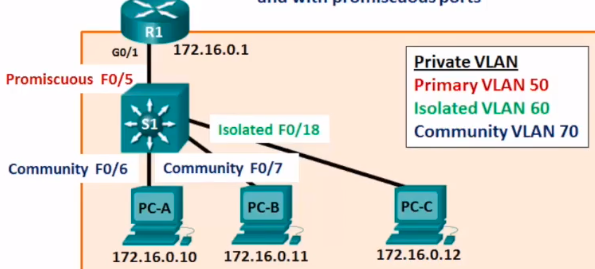
\includegraphics[scale=0.5]{pictures/PVLANconfig.PNG}
\end{figure}

\begin{sexylisting}{PVLAN}
vtp mode transparent

vlan 60
private-vlan isolated
vlan 70
private-vlan community
vlan 50
private-vlan primary
private-vlan association 60,70
exit

int f0/5
sw mode private-vlan promiscuous
sw private-vlan mapping 50 60,70
int f0/6
sw mode private-vlan host
sw private-vlan host-association 50 70
int f0/7
sw mode private-vlan host
sw private-vlan host-association 50 70
int f0/18
sw mode private-vlan host
sw private-vlan host-association 50 60
exit
\end{sexylisting}

If you only have a 2960 series switch and you do not have a multilayer switch, you can use the \code{sw protected} interface configuration command to achieve a similar result. Ports configured with this command is called Protected ports. Hosts connected to Protected ports will not be able to communicate with each other, but can only talk with un-Protected ports. 

\section{DHCP snooping}

\textbf{DHCP starvation} attack creates a DoS by leasing all available IP addresses. It is easy to mitigate DHCP starvation attacks using port security. \\

A \textbf{DHCP spoofing} attack occurs when a rogue DHCP server is connected to the network and provides false IP configuration parameters to legitimate clients. DHCP spoofing attacks can be mitigated using DHCP snooping on trusted ports. The general rule is that ports connected to hosts are untrusted, the other is trusted. Port connected to DHCP server must be trusted, otherwise DHCP service will not work.

\begin{figure}[hbtp]
\caption{Trusted and untrusted DHCP spoofing ports}\label{DHCPspoofing}
\centering
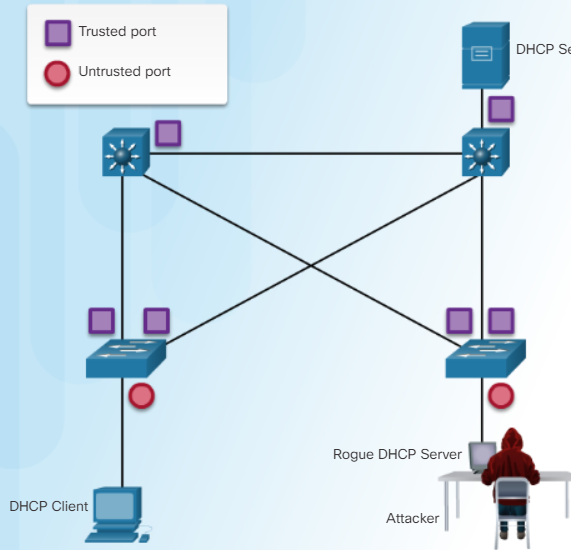
\includegraphics[scale=1]{pictures/DHCPspoofing.PNG}
\end{figure}

\begin{sexylisting}{DHCP snooping}
ip dchp snooping
 
int f0/1
ip dchp snooping trust
int range f0/5-24
ip dchp snooping rate 6
exit

ip dchp snooping vlan 5,10,20
\end{sexylisting}


\section{Dynamic ARP Inspection (DAI)}

An attacker can send a gratuitous ARP message containing a spoofed MAC address to a switch (ARP spoofing). \textbf{Dynamic ARP Inspection (DAI)} will be configured to mitigate against ARP spoofing and ARP poisoning attacks.

\begin{sexylisting}{Dynamic ARP Inspection (DAI) configuration}
ip dhcp snooping
ip dhcp snooping vlan 10
ip arp inspection vlan 10

int f0/24
ip dhcp snooping trust
ip arp inspection trust
exit

ip arp inspection validate src-mac
ip arp inspection validate dest-mac
ip arp inspection validate ip
ip arp inspection validate src-mac dest-mac ip
\end{sexylisting}

DHCP snooping is enabled because DAI requires the DHCP snooping table to operate. Next, DHCP snooping and ARP inspection are enabled for the PCs on VLAN10. The uplink port to the router is trusted, and therefore, is configured as trusted for DHCP snooping and ARP inspection.\\

The \code{ip arp inspection validate} global configuration command is used to configure DAI to drop ARP packets when the \code{ip}, or \code{src-mac} (source MAC address), or \code{dest-mac} (destination MAC address) are invalid. Notice that entering multiple \code{ip arp inspection validate} commands overwrite the previous command. To include more than one validation method, enter them on the same command line as displayed in the output.

\section{IP Source Guard (IPSG)}

To protect against MAC and IP address spoofing, configure the IP Source Guard (IPSG) security feature. IPSG operates just like DAI, but it looks at every packet, not just the ARP packets. Like DAI, IPSG also requires that DHCP snooping be enabled.\\

Specifically, IPSG is deployed on untrusted Layer 2 access and trunk ports using the \code{ip verify source} interface configuration command. IPSG dynamically maintains per-port VLAN ACLs (PVACL) based on IP-to-MAC-to-switch-port bindings. For each untrusted port, there are two possible levels of IP traffic security filtering:

\begin{itemize}
\item IP addresses -- only IP traffic with a source IP address that matches the IP source binding entry is permitted. 
\item IP and MAC address -- Only IP traffic with source IP and MAC addresses that match the IP source binding entry are permitted.
\end{itemize}

\section{Mitigating STP Attacks}

\subsection{PortFast}

The spanning-tree PortFast feature causes an interface configured as a Layer 2 access port to transition from the blocking to the forwarding state immediately, bypassing the listening and learning states. PortFast can be used on Layer 2 access ports that connect to a single workstation or server. Because the purpose of PortFast is to minimize the time that access ports must wait for STP to converge, it should be used only on access ports. \\

PortFast can be configured globally on all non-trunking ports using the \code{spanning-tree portfast default} global configuration command. Alternatively, PortFast can be enabled on an interface using the \code{spanning-tree portfast} interface configuration command.

\subsection{BPDU Guard}

Even though PortFast is enabled, the interface will listen for BPDUs. The receipt of unexpected BPDUs might be accidental, or part of an unauthorized attempt to add a switch to the network. BPDU Guard protects the integrity of ports that are PortFast-enabled. If any BPDU is received on a BPDU Guard enabled port, that port is put into error-disabled state. \\

Use the \code{spanning-tree portfast bpduguard} default global configuration command to globally enable BPDU guard on all PortFast-enabled ports. If PortFast is not configured, then BPDU Guard is not activated. Alternatively, BPDU Guard can be enabled per interface using the \code{spanning-tree bpduguard enable} interface configuration command.

\note Always enable BPDU Guard on all PortFast-enabled ports.

\subsection{Root Guard}

On a network, there are some switches that should never, under any circumstances, become the STP root bridge. Root Guard provides a way to enforce the placement of root bridges on the network by limiting which switch can become the root bridge. \\

Root guard is deployed on ports that \emph{toward} the unsecure switches (switches that should not be the root bridge). Look at figure \ref{RootLoopGuard}, we don't want S1 to be root bridge, so that F0/1 on both S2 and S3, which are towards S1, should be configured with Root Guard.\\
If a root-guard-enabled port receives BPDUs that are superior to those that the current root bridge is sending, that port is moved to a \emph{root-inconsistent state}. Recovery occurs as soon as the offending device ceases to send superior BPDUs.\\

\begin{figure}[hbtp]
\caption{Root and Loop Guard reference topology}\label{RootLoopGuard}
\centering
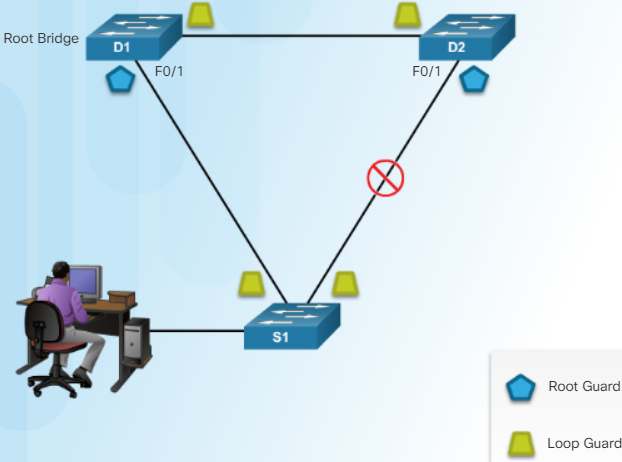
\includegraphics[scale=1]{pictures/RootLoopGuard.PNG}
\end{figure}


Use the \code{spanning-tree guard root} interface configuration command to configure root guard on an interface. To view Root Guard ports that have received superior BPDUs and are in a root-inconsistent state, use the \code{show spanning-tree inconsistent ports} command.

\subsection{Loop Guard}

Traffic on bidirectional links flows in both directions. If for some reason one direction traffic flow fails, this creates a unidirectional link which can result in a Layer 2 loop. If BPDUs are not received on a non-designated Loop Guard-enabled port, the port transitions to a loop-inconsistent blocking state, instead of the listening / learning / forwarding state. \\

Loop Guard is enabled on all \emph{non-Root guard} ports (figure \ref{RootLoopGuard}) using the \code{spanning-tree guard loop} interface configuration command.